\section{Event and Kinematic Selection}

\subsection{Event selection}

%  updated by Erez on Jan 11

The analysis selection uses reconstructed objects from both the P$\emptyset$D
and TPC. Both sub-detectors use independent reconstruction algorithms
to generate objects from the raw data. The P$\emptyset$D uses a 3D tracking
algorithm to form tracks from individual hits in the scintillator
bars. The TPC reconstruction uses a track in the Y-Z plane (non-drift plane)
as a seed to search for hits in the downstream FGD to form a track object.
\begin{figure*}
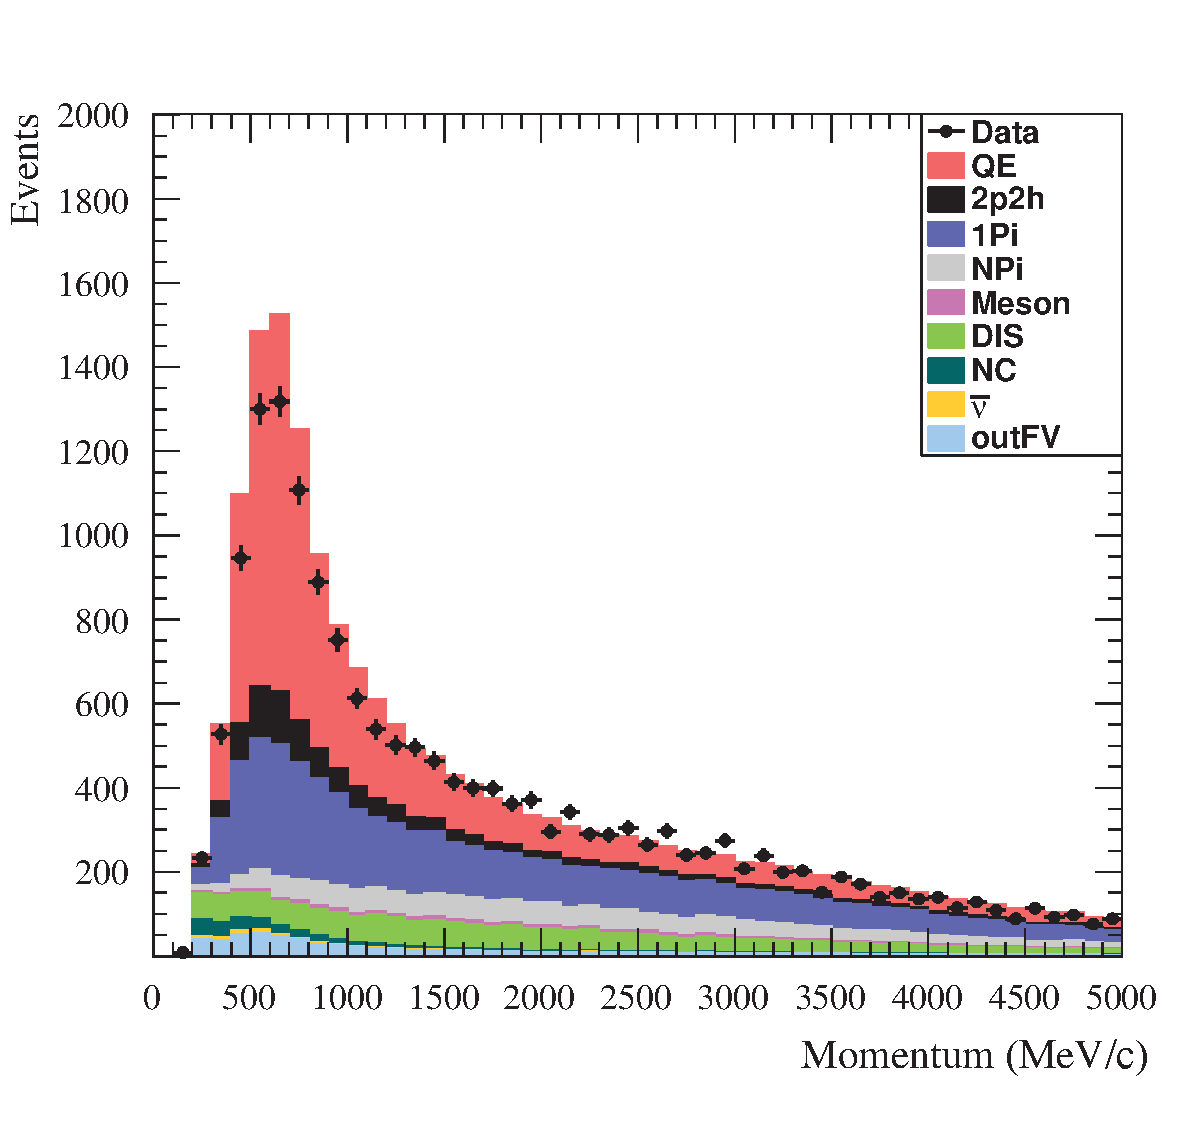
\includegraphics[scale=0.29]{P0DTrackerMom-MC6BRun4water-Data6BRun4water-ByRCode-v2} 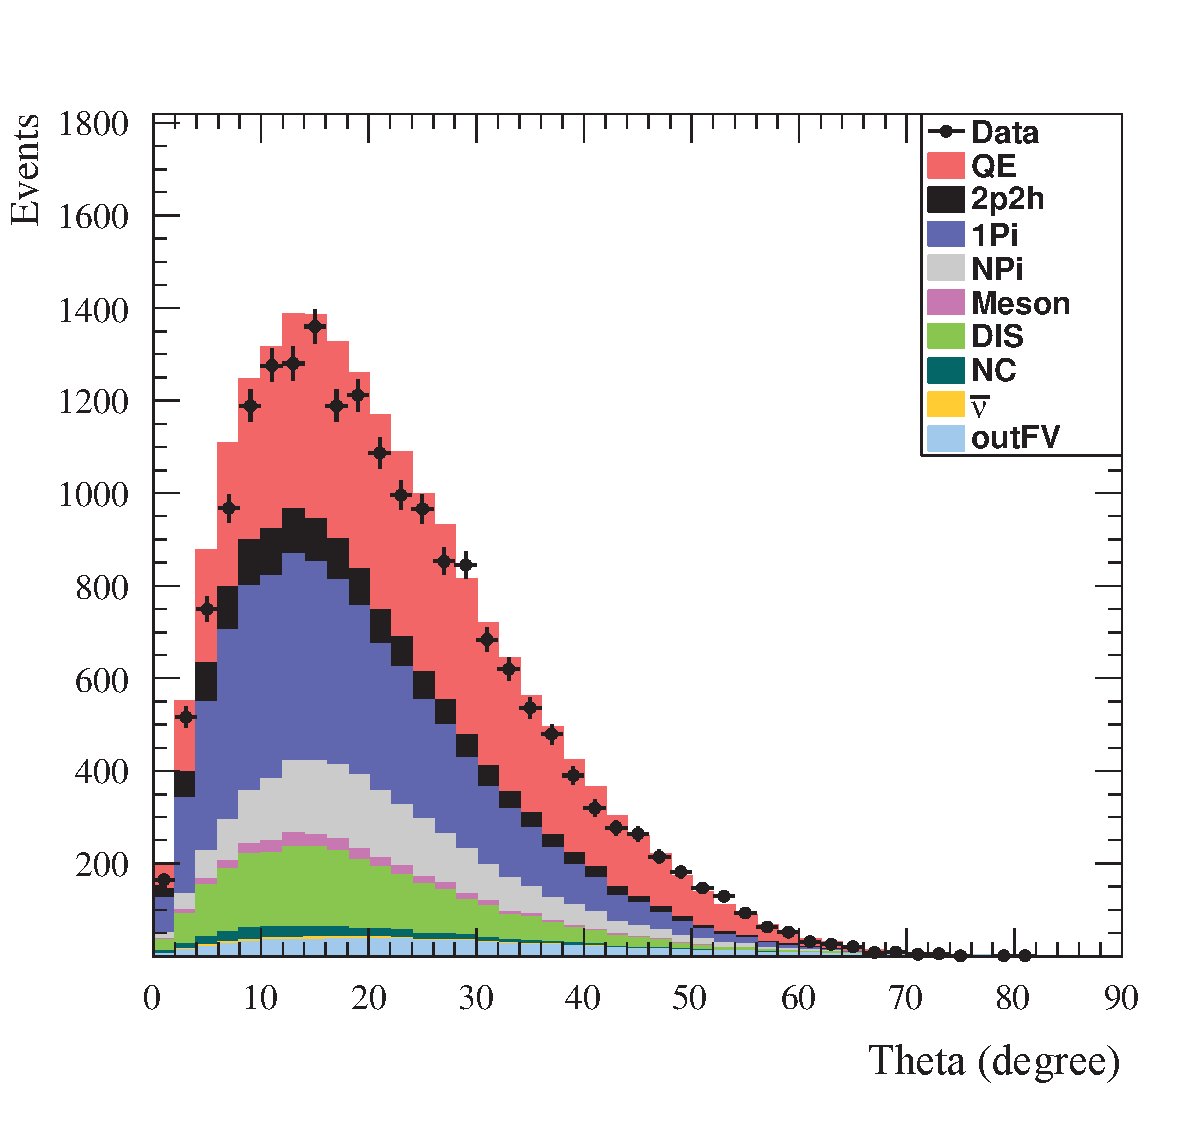
\includegraphics[scale=0.29]{P0DTrkTheta-MC6BRun4water-Data6BRun4water-ByRCode-v2} 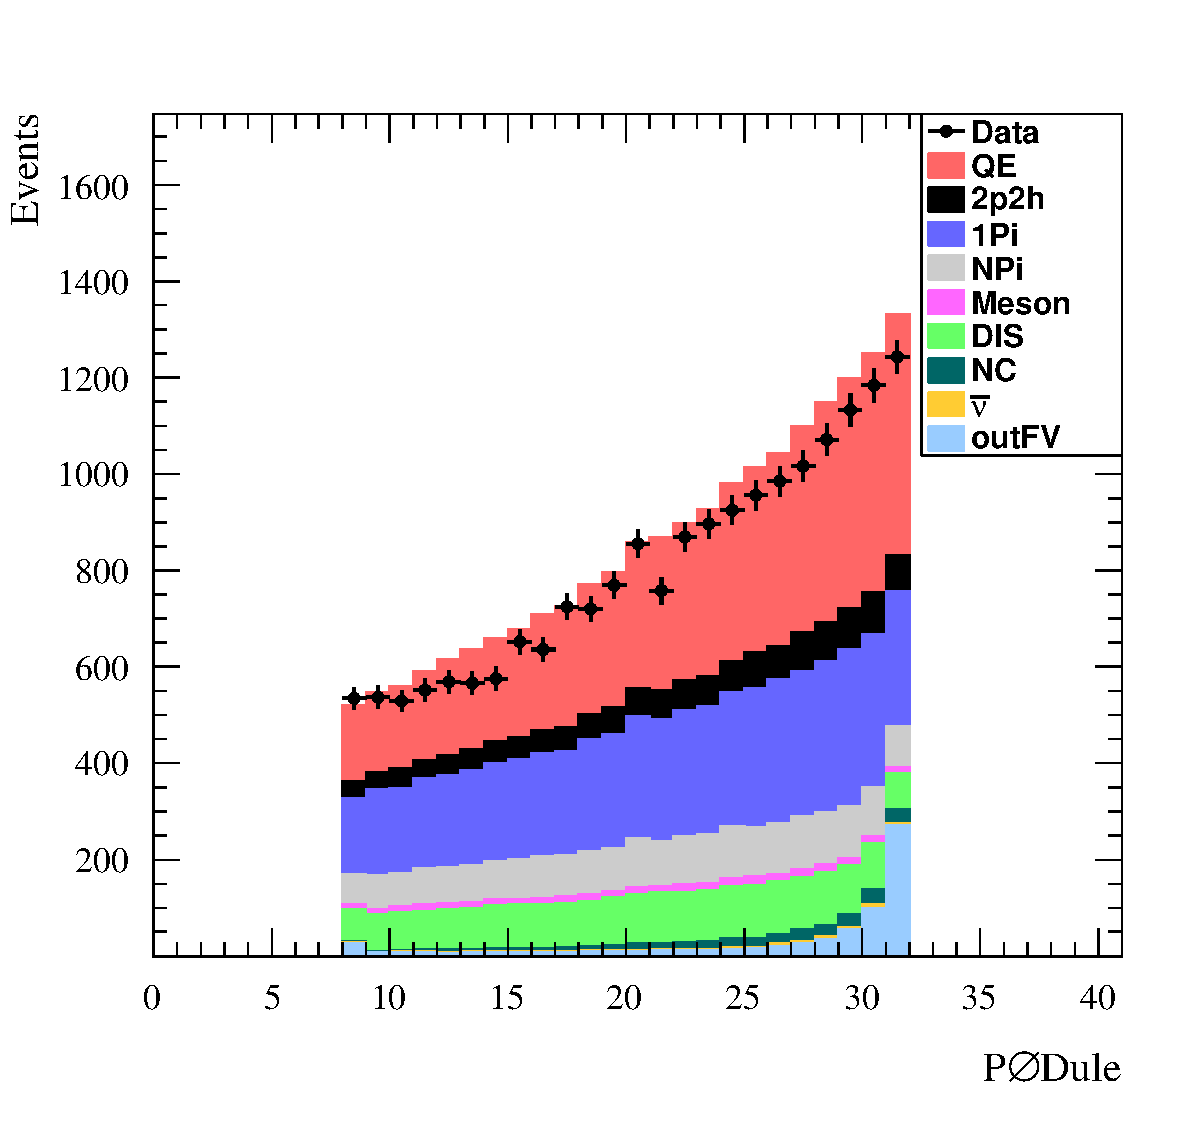
\includegraphics[scale=0.29]{P0Dule-MC6BRun4water-Data6BRun4water-ByRCode}

\caption{\label{fig:FHC-Neutrino-beam}FHC beam CCINC $\nu_\mu$ event
candidate distributions of the $\mu^{-}$ momentum in MeV/c
(Left), the muon $\theta_{\mu}$ angle in degrees (Middle), and interaction
vertex position by P$\emptyset$Dule (Right). Note backgrounds in the
CCINC sample are the NC (dark green), $\bar\nu_\mu$ induced events (yellow)
and the out of fiducial volume events (light blue).
There are negligible $\bar\nu_\mu$ backgrounds (yellow)
in the FHC sample.}
\end{figure*}

\begin{figure*}
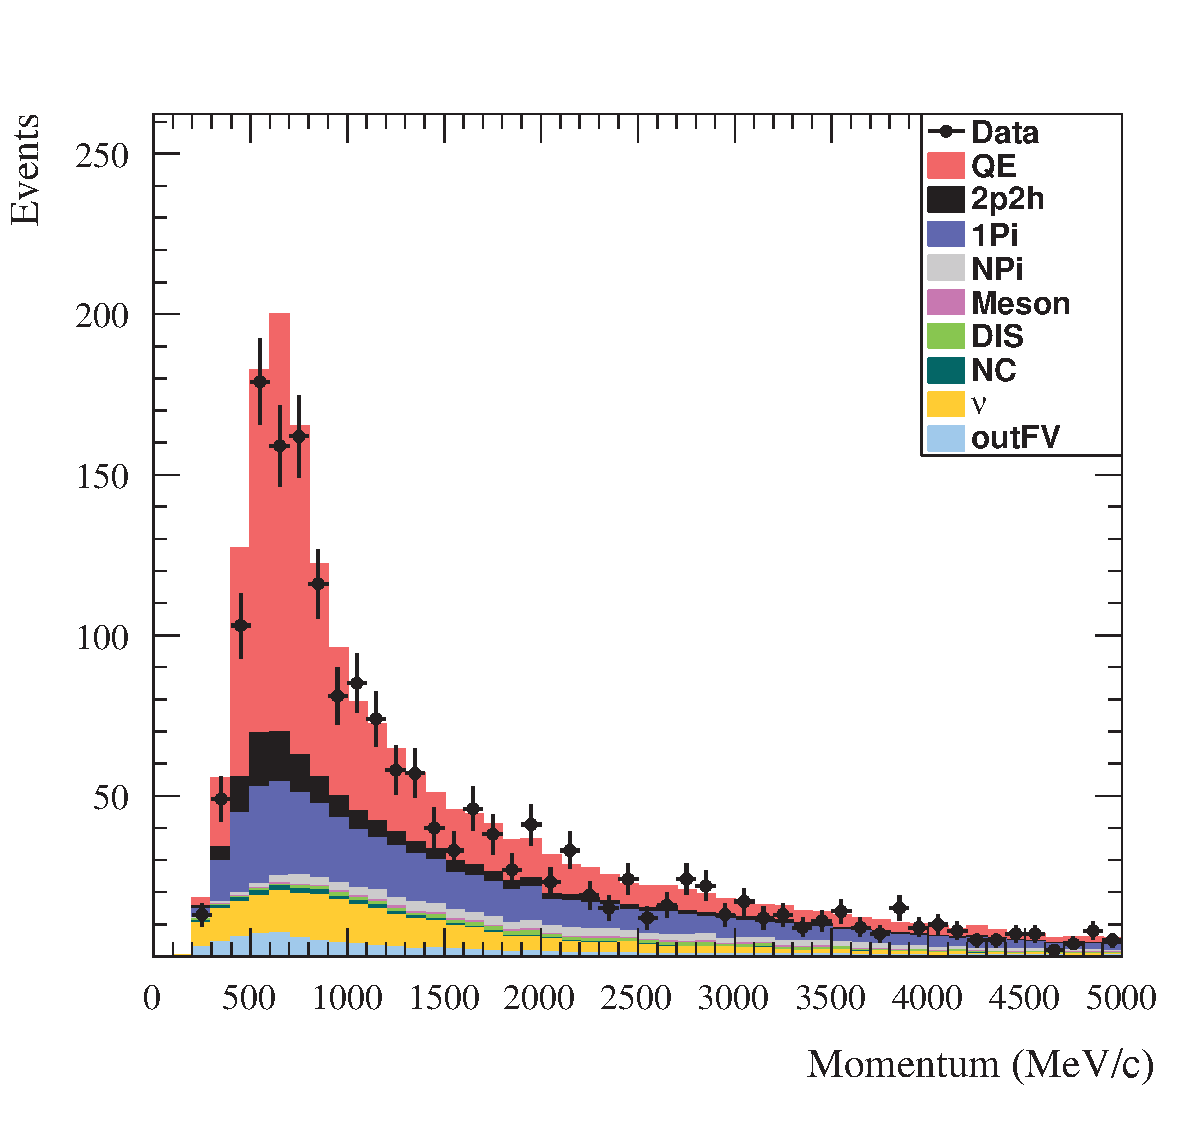
\includegraphics[scale=0.29]{P0DTrackerMom-MC6BRun5waterAnti-Data6CRun5waterAnti-ByRCode-v2}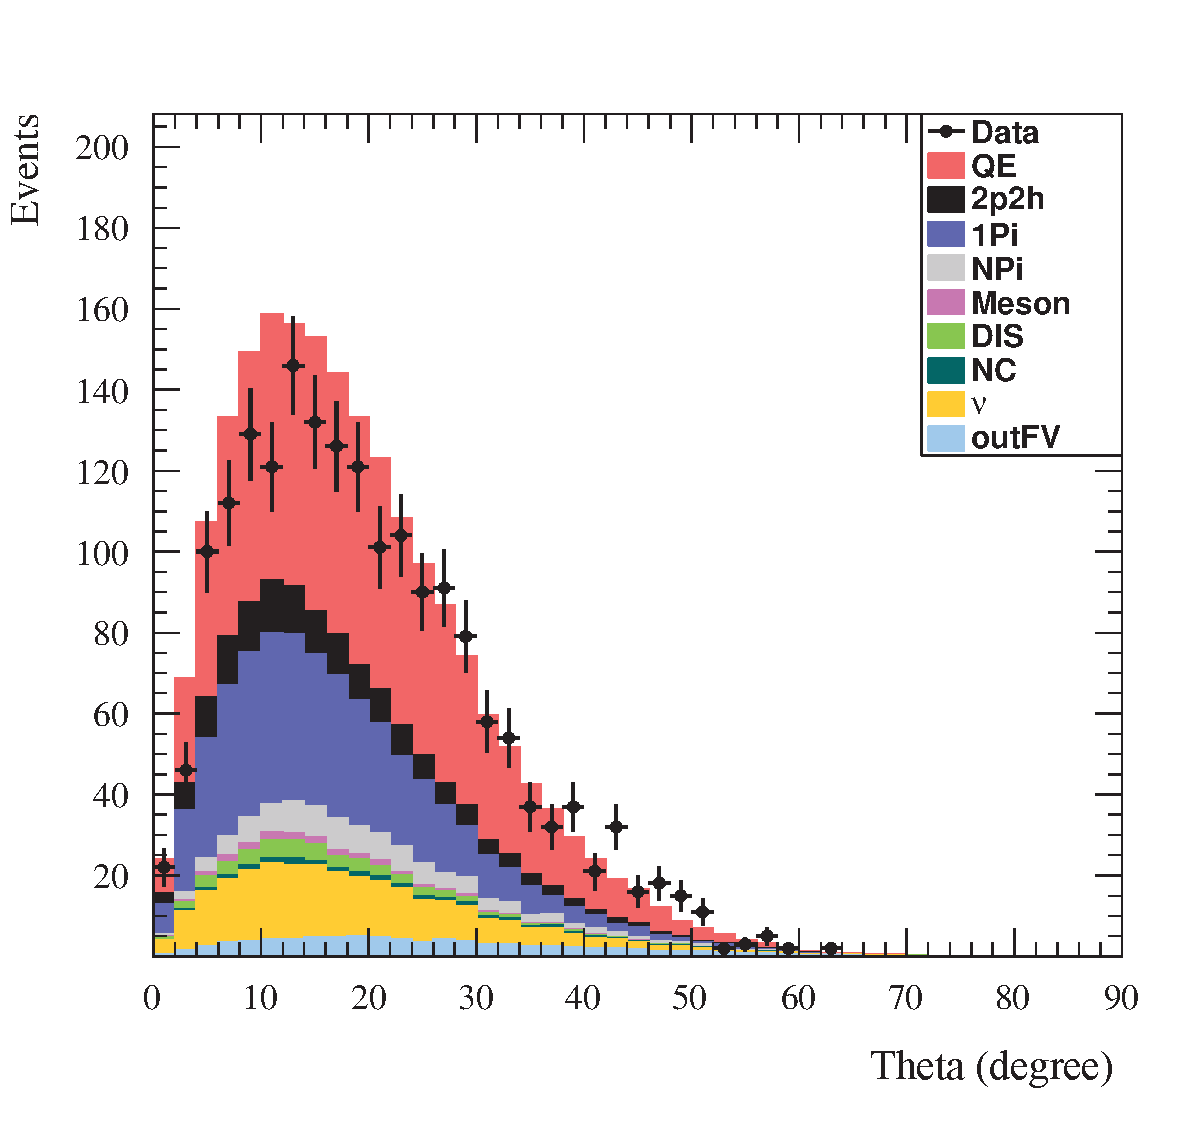
\includegraphics[scale=0.29]{P0DTrkTheta-MC6BRun5waterAnti-Data6CRun5waterAnti-ByRCode-v2}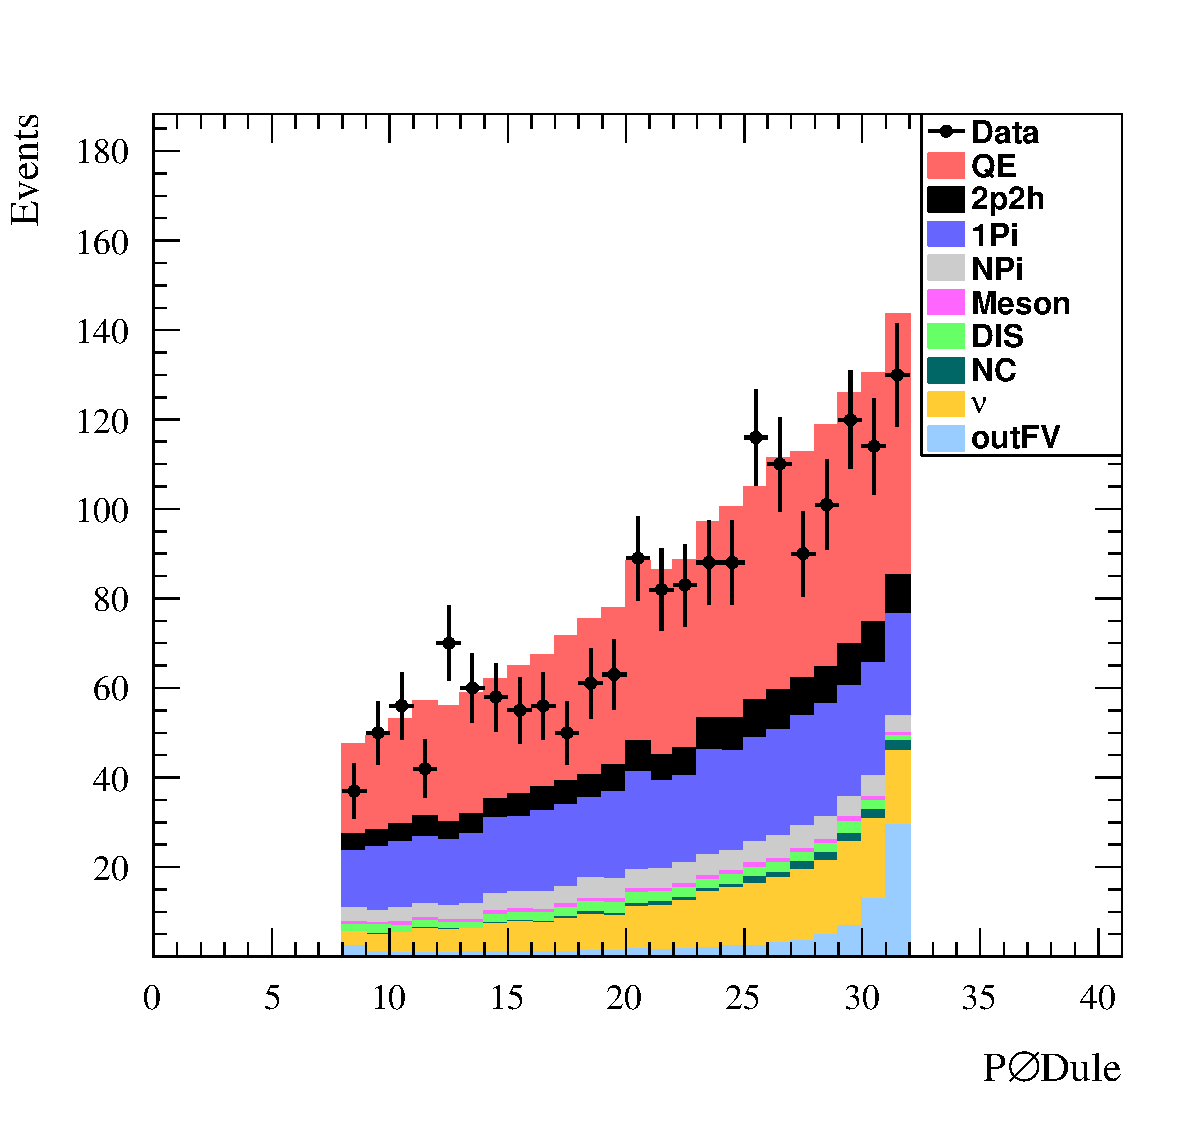
\includegraphics[scale=0.29]{P0Dule-MC6BRun5waterAnti-Data6CRun5waterAnti-ByRCode}


\caption{\label{fig:RHC-antineutrino-beam}RHC beam CCINC \nubar
event candidate distributions of the $\mu^{+}$ momentum in MeV/c
(Left), the muon $\theta_{\mu}$ angle in degrees (Middle), and interaction
vertex position by P$\emptyset$Dule (Right). 
Note backgrounds in the
CCINC sample are the NC (dark green), $\nu_\mu$ induced events (yellow)
and the out of fiducial volume events (light blue). The $\nu_\mu$ backgrounds
in the RHC beam sample are much larger than the analogous $\bar\nu_\mu$ backgrounds
in the FHC beam sample.}
\end{figure*}

After independent reconstructions in the TPC and in the P$\emptyset$D, the analysis
uses an algorithm to match a 3D P$\emptyset$D track ending
near the most downstream edge of the P$\emptyset$D to a TPC track beginning
near the most upstream edge of the TPC.

The event selection is the following: 
\begin{enumerate}
\item The first requirement is good data quality for the data run.
After ND280 data is processed, the sub-detectors are evaluated 
run by run for
good timing with respect to the beam and 
checked to satisfy good detector calibrations.
%proper gains.
Events are used only if their run passed data quality checks.
For each FHC (RHC) 
beam bunch there must be a negative (positive) TPC track
that is identified within $\pm$70~ns around the
nominal beam bunch time. 

\item A veto is applied to reject events whose vertex originated
outside the fiducial region but had a secondary interaction
inside the fiducial region. Also events with
single tracks that are broken into two tracks by the track reconstruction
are rejected. The event vertex is defined by the most upstream P$\emptyset$Dule
hit in the track. The vertex X-Y position is defined by the X-Y triangular
scintillator bars and the vertex Z position of the P$\emptyset$Dule. The fiducial
volume requires the vertex to be within -836 mm\ $<X<$ 864 mm and
-871 mm\ $<Y<$ 869 mm and inside one of the middle 24 P$\emptyset$Dules. 
The X boundaries are $\sim 250$ mm and the Y boundaries are
$\sim 236$ mm away from the ends of the X and Y scintillator bars, respectively.
%(out of 40). 
\item The vertex must be in the
P$\emptyset$D water target fiducial volume. The charge is determined by the
curvature of the TPC track. Of all TPC tracks meeting these criteria, the
one with the highest reconstructed momentum at the start of the track
is chosen to be the lepton candidate. 
\item The RHC mode selection has an additional requirement
that the lepton track candidate is positively charged
and has the highest momentum of all 
charged tracks in the bunch.
\end{enumerate}

Due to the limited geometric acceptance of requiring a CC neutrino event vertex in the  P$\emptyset$D with
its muon track detected in the TPC, this analysis is inherently not sensitive to the
entire muon kinematic phase space. For this reason, we define a restricted
phase space, described in the next sub-section, that will cover the
part of the kinematic phase space where we have good acceptance.
Events that are reconstructed to have muon kinematics outside of the
restricted phase space will be rejected.
\begin{table}

\caption{%The fractional distribution of true MC interactions for the 
The fractional distributions of true MC interactions for selected events
defined at the initial interaction vertex according to the NEUT generator for the 
FHC beam (Left) and RHC beam (Right) modes. See text for descriptions
of each MC channel.\label{tab:The-fractional-distribution-1}}

\begin{tabular}{lc}
\hline 
\hline
\multicolumn{2}{c}{FHC beam}\\ % \tabularnewline
\hline 
Mode & Fraction \\
\hline 
QE & 37.83\% \\ %\tabularnewline
2p2h & 3.30\% \\ %\tabularnewline
1Pi & 29.73\% \\ %\tabularnewline
NPi & 11.01\% \\
Meson & 1.71\% \\
DIS & 11.27\% \\
NC & 1.50\% \\
$\overline{\nu}_{\mu}$ & 0.33\% \\
outFV & 3.32\% \\
\hline 
\hline
\end{tabular}\ %
\begin{tabular}{lc}
\hline 
\hline
\multicolumn{2}{c}{RHC beam}\tabularnewline
\hline 
Mode & Fraction\tabularnewline 
\hline 
QE & 47.27\%\tabularnewline
2p2h & 3.19\%\tabularnewline
1Pi & 24.14\%\tabularnewline
NPi & 5.05\%\tabularnewline
Meson & 1.04\%\tabularnewline
DIS & 2.32\%\tabularnewline 
NC & 0.99\%\tabularnewline 
$\nu_{\mu}$ & 11.93\%\tabularnewline 
outFV & 4.05\%\tabularnewline
\hline
\hline 
\end{tabular} 
\end{table}
For the FHC mode selection, 19,259 events are selected in data.
The number of selected events in the corresponding MC sample,
scaled to the same data PoT exposure is 19,566. In RHC mode,
1,869 events are selected in data and the scaled MC sample has 1,953 events. 
%These event numbers are listed in Table VI as the
%full phase space (PS) samples.
The muon $p$ and $\theta$ distributions for data events with MC predictions 
are shown for both modes
in  Figs. \ref{fig:FHC-Neutrino-beam} (Left and Middle) and
\ref{fig:RHC-antineutrino-beam} (Left and Middle), respectively. The plots 
include colored stacked histograms 
of MC interaction types to graphically display the composition
of the selected events. 

The fractional NEUT interaction types for the FHC and the
RHC beam modes are given in Table \ref{tab:The-fractional-distribution-1}
for the selected events described in Section IV. The MC channels defined\citep{joe-sam}
at the
initial interaction vertex according to NEUT are 
CCQE (QE), 2p2h, CC with 1 charged pion (1Pi), CC with
>1 charged pion (NPi), CC with K or $\eta$ meson (Meson), deep inelastic
scattering (DIS), neutral current (NC),
neutrino or antineutrino interaction
($\nu$ or $\overline{\nu}$), and events whose true vertex position was
outside the fiducial volume (outFV) region of the P$\emptyset$D . The 
resulting selected events, according to the MC simulation, 
are predominately CCQE, followed by CC events with 1 pion. 
%In addition, the fraction of CCQE events and the fraction of those
%events of the charged current process
%that has no pions (CC0$\pi$) before selection cuts in the generated neutrino CCINC event sample were
%determined to be  $47.8\%$ and $59.8\%$, respectively.  
Due to a substantial
$\nu_\mu$ flux contamination in the RHC beam and a large $\nu_\mu$ cross section,
the \nubar candidate sample has a larger background fraction (see yellow band
in Fig. \ref{fig:RHC-antineutrino-beam})
compared to the $\bar{\nu}_\mu$ background events in the FHC
beam sample. 
The $\nu_\mu$ in the
RHC beam flux is seen in Fig.\ref{fig:The-neutrino-FHC} (Bottom). 
The outFV backgrounds are roughly the same
fraction in both FHC and RHC beam samples. The selection 
produces a CCINC $\nu_\mu$ candidate event sample that is 94.8\% pure 
and a CCINC $\bar\nu_\mu$ cadidate event sample that is 83.0\% pure. 
%The CCinc signal events are predominantly CCQE and 1-pion. 
The outFV backgrounds cluster in
the light blue bands in Figs. 
\ref{fig:FHC-Neutrino-beam} (Right) 
and
\ref{fig:RHC-antineutrino-beam} (Right) 
in the downstream P$\emptyset$Dules. These backgrounds are events whose 
vertices are outside and downstream of the fiducial volume but with 
an interaction that has a backwards going
track that enters the fiducial volume.
%The RHC sample includes a non-negligible background neutrino component 
%which is caused by a large fraction of $\nu_\mu$ in the
%RHC beam flux as seen in Fig.\ref{fig:The-neutrino-FHC} (Bottom). 

Additional checks between the data and MC event selections were performed by
comparing the event rates of vertices by detector P$\emptyset$Dule between data
and normalized selected MC events. The event rates by P$\emptyset$Dule are shown
for \nuandnubar
in the Figs. \ref{fig:FHC-Neutrino-beam} (Right) and \ref{fig:RHC-antineutrino-beam}
(Right), respectively. There is very good
agreement within statistics between the data and MC distributions, except the
momentum distribution in the FHC beam sample where the data is
1-2 sigma below the MC predictions near 0.6 GeV/c. 
The efficiency for the \nuandnubar events varies as a function of P$\emptyset$Dule.
Since the event selection requires a vertex in a P$\emptyset$Dule with a muon track
reconstructed in the TPC, the downstream P$\emptyset$Dules have a higher
efficiency than the upstream P$\emptyset$Dules. The events with vertices
in the more upstream P$\emptyset$Dule have smaller angular acceptance for
a muon track to pass through the TPC and the muon track will incur
more energy loss since it must pass through more P$\emptyset$Dules to reach
the TPC where it must be reconstructed. The $\nu$ event selection
efficiency in Fig. \ref{fig:FHC-Neutrino-beam} (right) from upstream
to downstream P$\emptyset$Dule varies from 37\% to 57\% whereas the \nubar
event selection efficiency Fig. \ref{fig:RHC-antineutrino-beam} (right)
varies from 39\% to 68\%. 
%The positive helicity \nubar interaction
%has a higher efficiency since the $\mu^{+}$ is more forward going than
%the $\mu^{-}$ from the negative helicity neutrino interaction.

%\iffalse
\begin{figure*}
%\includegraphics[scale=0.8]{generate-full_CCinc}
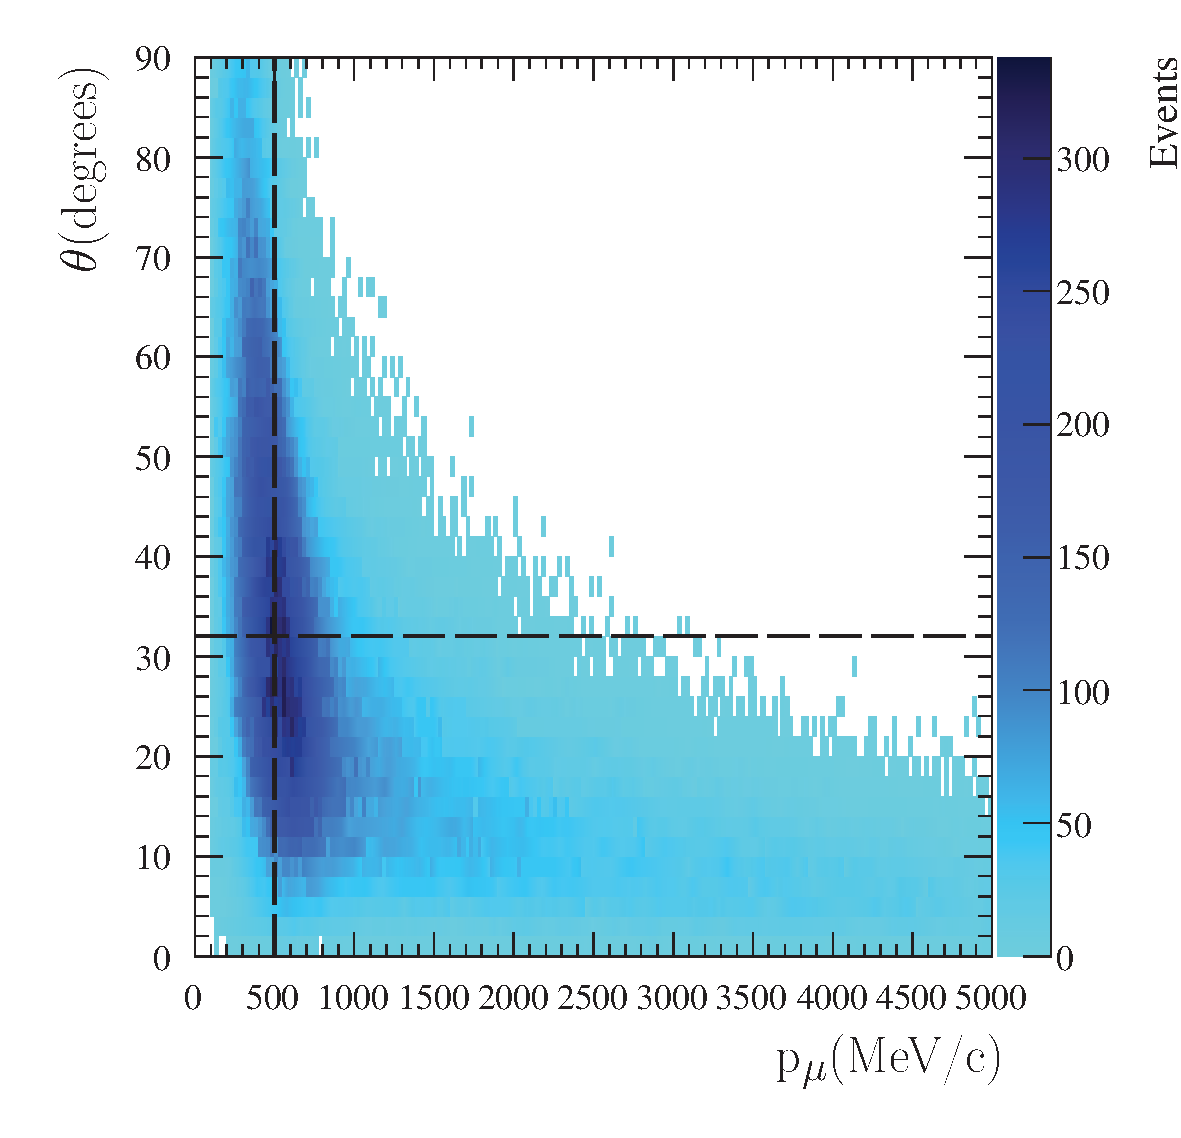
\includegraphics[scale=0.35]{Panh2GenThetaGenMomentumRun5waterAnti-v2}
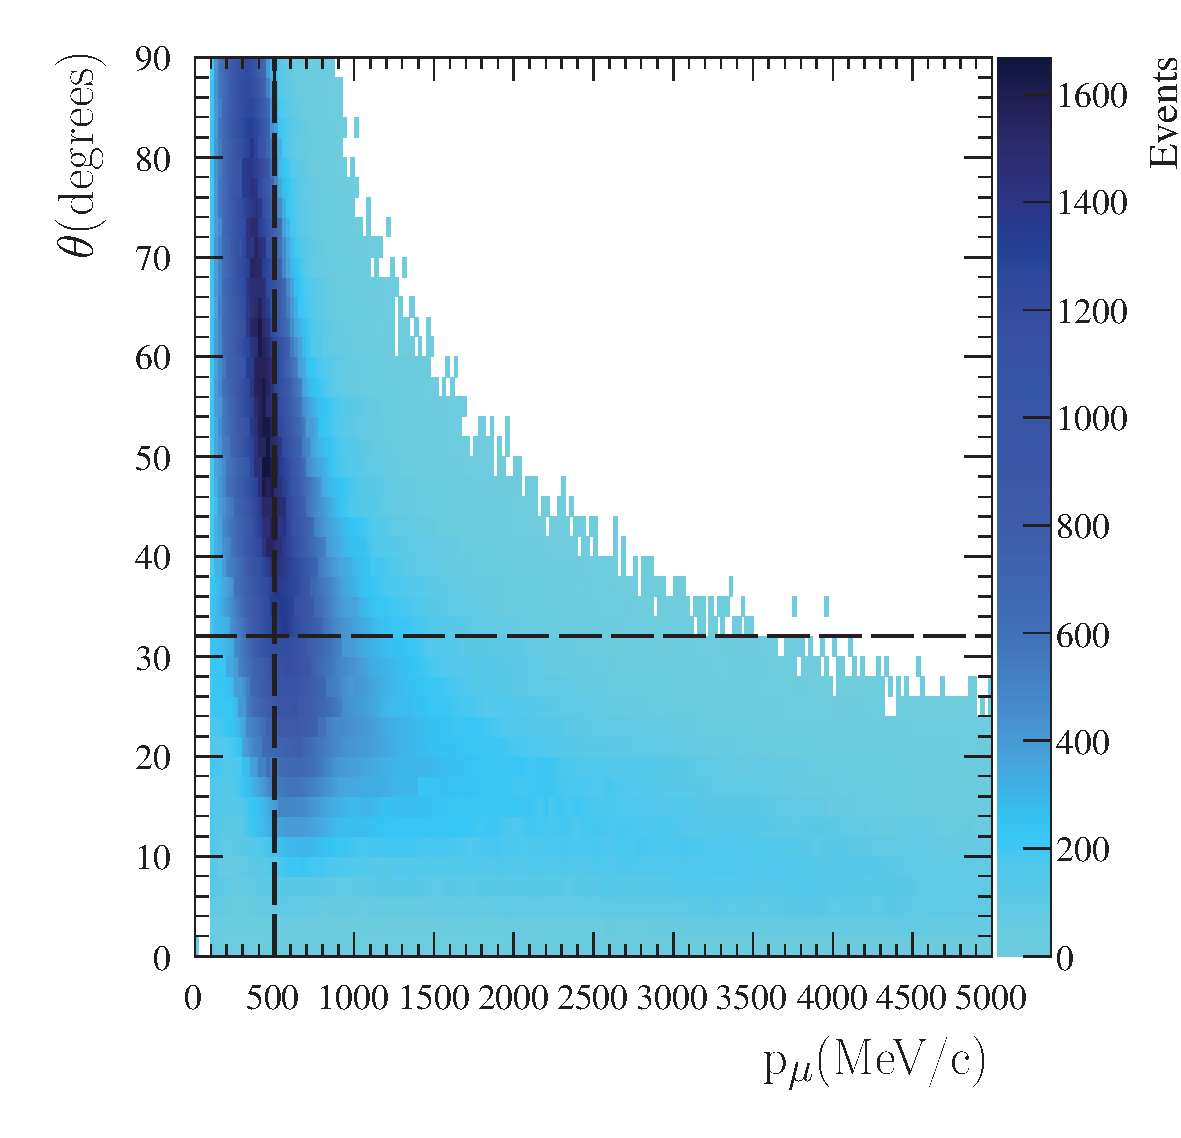
\includegraphics[scale=0.35]{Panh2GenThetaGenMomentumRun4water-v2}
\caption{\label{fig:full-CCinc-generated}
Left (Right) 2-D plots of  $\theta_{\mu}$ versus $p_{\mu}$
for RHC (FHC) beam events of $\mu^{+}\left(\mu^{-}\right)$
tracks using MC generated CCINC with full acceptance. The vertical
and horizontal solid lines correspond to %{\color{blue} 
$\theta_{\mu}=32\protect\textdegree$
and $p_{\mu}=500$ MeV/c, respectively. 
} 
\end{figure*}
 %\fi

\begin{figure*}
%\includegraphics[scale=0.8]{P0D+TPC-mc_events}
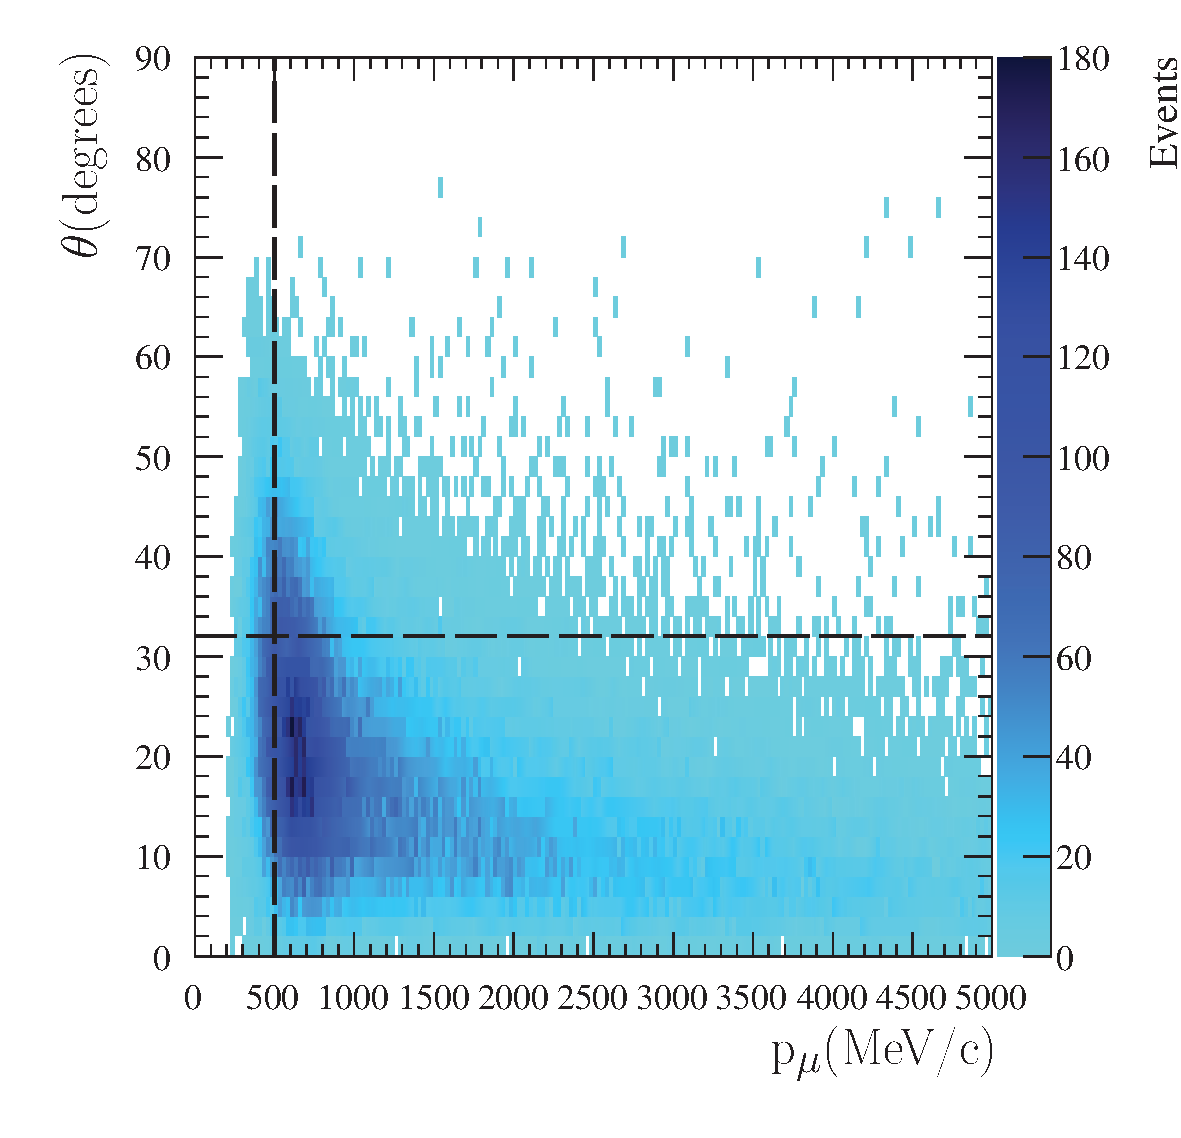
\includegraphics[scale=0.35]{Panh2RecoMuThetaRecoMomentumRun5waterAnti-v2}
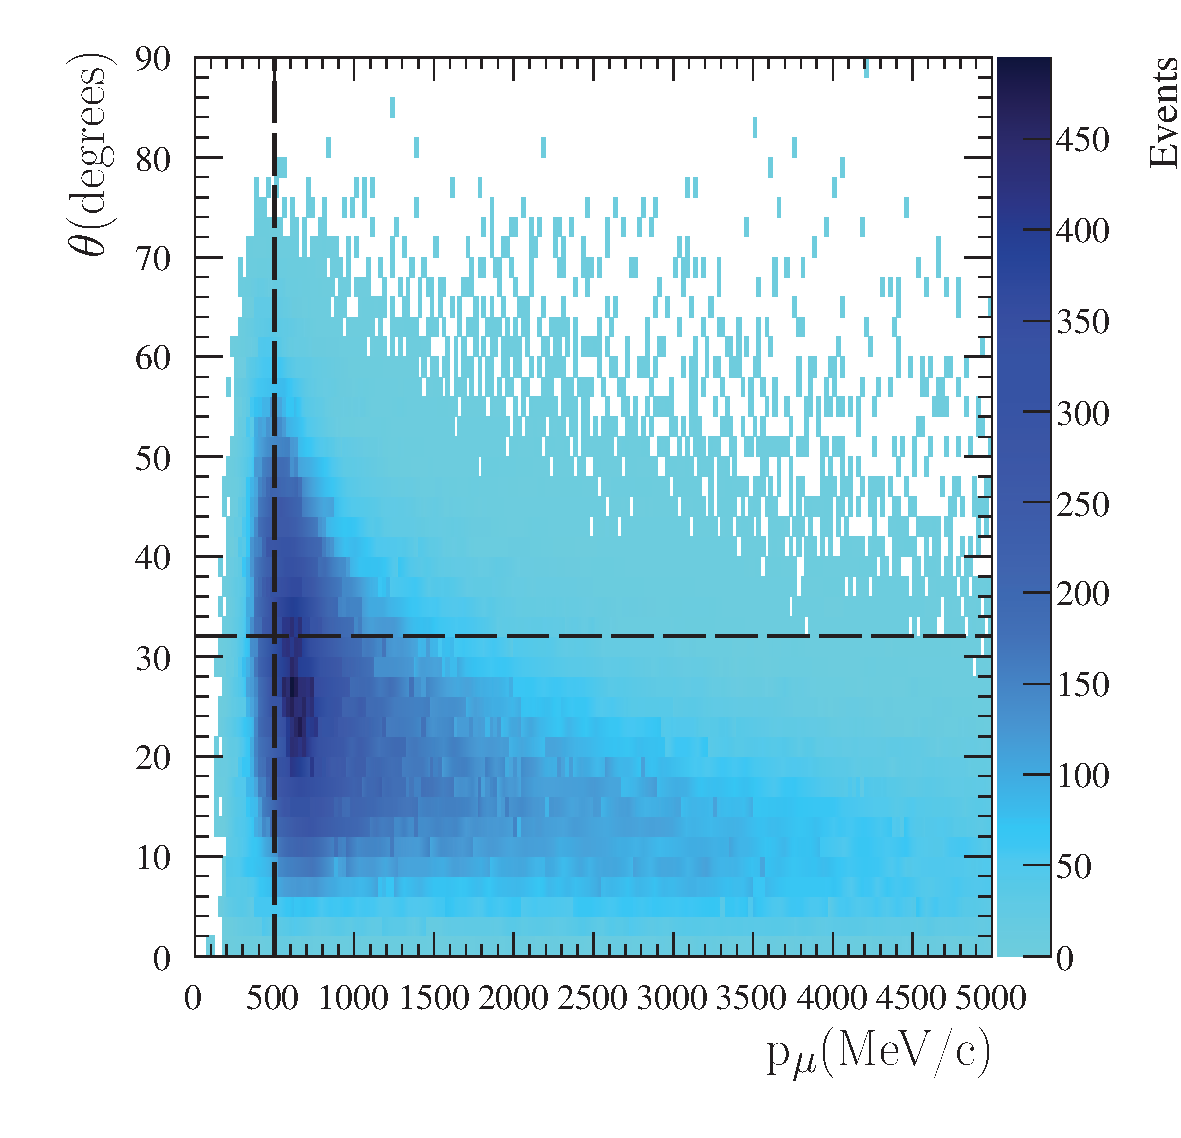
\includegraphics[scale=0.35]{Panh2RecoMuThetaRecoMomentumRun4water-v2}

\caption{\label{fig:P0D-vertex-and} Left (Right) 2-D plots of  $\theta_\mu$ versus $p_\mu$ 
for RHC (FHC) beam events of $\mu^+\left(\mu^-\right)$
tracks using MC generated CCINC that have a reconstructed P$\emptyset$D vertex and TPC muon
track. The vertical and horizontal solid lines correspond to 
$\theta_\mu=32\protect\textdegree$
and $p_\mu=500$ MeV/c, respectively. The restricted phase space
cut selection applies to events inside the
lower right
rectangular region 
defined by the dashed lines. }
\end{figure*}

\subsection{Kinematic selection}

The selected events for the RHC (FHC) samples require a vertex in
the P$\emptyset$D and a $\mu^{+}\left(\mu^{-}\right)$ reconstructed track in
the TPC detector. 
%{\color{blue}
This limits or restricts the available kinematic
phase space of the CCINC events such that
certain kinematic regions are not measured. 
These unmeasured regions in the laboratory frame
have low muon momentum 
$p_\mu<500$ MeV/c or large muon polar angles
$\theta_{\mu}>32\textdegree$.

These kinematic boundaries are displayed in Figs. \ref{fig:full-CCinc-generated}
and \ref{fig:P0D-vertex-and} Left (Right)
where the  $\theta_{\mu}$ versus $p_{\mu}$
2-D plots are shown for the RHC (FHC) samples. In Fig.
\ref{fig:full-CCinc-generated} Left (Right) are the generated MC
full acceptance CCINC events for the RHC (FHC) samples. The $\nu_\mu$
mode has more events with larger $\theta_{\mu}$ polar angles since
the $\mu^{-}$ angular distribution is more isotropic than the $\mu^{+}$
in the \nubar mode whose muon tracks are more forward. 
%and peaked at $\theta_{\mu}=0$. 
In Fig. \ref{fig:P0D-vertex-and} Left (Right)
are the generated MC CCINC events that have a P$\emptyset$D vertex and a $\mu^+$ ($\mu^-$)
track reconstructed in the TPC for the RHC (FHC) samples. The regions
below horizontal lines  where $\theta_{\mu}<32\textdegree$ and right of
the vertical dash lines where $p_\mu>500$ MeV/c are detector regions
that have non-zero acceptance
and reconstructed events for both the
FHC and the RHC samples.
Hence we use these two kinematic
restrictions in the cross section measurements.
%\[
%\begin{array}{c}
% 
%{\color{blue} p_{\mu}>500MeV/c }\\
%\\
%{\color{blue} \theta_{\mu}<32} \textdegree 
%
%\end{array}
%\]
The resulting 
reconstructed
restricted phase space selection in
the $\nu_\mu$ mode has 14,398 data events and 
a corresponding MC sample, scaled to the same
data PoT exposure, contains 15,284 events. In the \nubar
mode, 1,461 data events are selected and a scaled MC sample
has 1,634 events. From a study of MC truth selected events, this restricted
phase space selection changed the mean value of 
neutrino energies below 2 GeV in the FHC sample from
0.83 GeV (unrestricted) to 1.14 GeV (restricted) 
and in the RHC sample from 0.84 GeV (unrestricted) to 1.08 GeV (restricted). 
In addition, the $\nu_\mu$ and  \nubar MC samples
contained 2.19\% and 1.33\% events, respectively, 
whose true kinematic value was outside the restricted phase
space region, but its reconstructed value migrated to be 
inside the restricted phase space region.
These events are kinematic backgrounds that originated
from the same physics process. 



